\documentclass{article}

\usepackage[ngerman]{babel} 

\usepackage[T1]{fontenc}
\usepackage{lmodern}
\usepackage[utf8]{inputenc}
\usepackage{graphicx}
\usepackage{amsmath}
\usepackage{amssymb}
\usepackage{amsthm} 
\usepackage{wasysym}
\usepackage[justification=centering]{caption}
\usepackage[parfill]{parskip}
\usepackage[left=3cm,right=3cm,top=2cm,bottom=2cm,includeheadfoot]{geometry}
\usepackage{subfig}
\usepackage{units}
\usepackage{subscript}
\usepackage[ruled,german]{algorithm2e}
\usepackage{textcomp}
\usepackage{tikz}
\usepackage{url}
\usetikzlibrary{shapes}

\newtheorem{satz}{Satz} 

\newcommand{\BigO}[1]{\ensuremath{\operatorname{O}\left(#1\right)}}
\newcommand{\subs}[2]{#1\textsubscript{#2}}

\usepackage[sortcites=true, style=alphabetic,natbib=true]{biblatex}

\bibliography{bibliography}

%Autornamen in Bibliography fett
\AtBeginBibliography{\renewcommand*{\mkbibnamelast }[1]{\textbf{#1}}}
\AtBeginBibliography{\renewcommand*{\mkbibnamefirst }[1]{\textbf{#1}}}


\begin{document}
% Title page

% ############################################
\section{Problembeschreibung und -analyse}

\subsection{Problembeschreibung}

Die Hauptschwierigkeit des Problems liegt daran, dass es sich eigentlich
um eine Kombination aus (mindestens) zwei Problemen handelen. Jedes Problem
für sich ist gut beschrieben und gelöst worden, doch für alles gleichzeitig
nicht.

\begin{enumerate}
\item Graph coloring - Visit stuff
\item Evacuate 
\end{enumerate}

\subsection{Annahmen über das Problem}

\begin{itemize}
\item Roboter sind punktförmig
\item Können in der Bewegung saugen
\item Keine Beschränkung, wie viele Roboter sich in einem Punkt befinden
\item Kommunikation ist instantan und ohne Berechnungszeit (Senden wie Empfangen)
\item Kommunikation zwischen Robotern kann alles sein
\item Roboter haben unbeschränkt viel Speicher
\end{itemize}

\subsection{Disclaimer}

Einschränkungen nicht simuliert, aber deren Auswirkungen

% ############################################
\clearpage
\section{Vorgehensmodell}

\begin{itemize}
\item Keep it simple
\item Start with working prototype before you do srs stuff
\item Getrennt marschieren, zusammen kämpfen (self contained subprograms, assemble at the end, bottom to top)
\item ipython notebook
\item using a lib before reinventing the wheel
\item Optimize when needed, first correct and working, then fast
\item 90 \% thinking, 10 \% coding
\item Abstract away decisions not made or which might change (geometry, polygon, agent)
\end{itemize}

\subsection{Design-Ziele}

\subsection{Nicht-Ziele}

Schöne UI, nur usable

% ############################################
\clearpage
\section{Problembetrachtung}

Das Problem kann unter vielen verschiedenen betrachtet 
werden. Je nachdem, in welcher Domäne der Informatik
es eingeordnet wird, gibt es unterschiedliche Lösungsansätze.

In diesem Abschnitt wird kurz beschrieben, welche Ansätze
erdacht wurden, welches deren Vor- und Nachteile sind, und
für welche schließlich ausgewählt wurden.

\subsection{Graphenproblem}

Suche

\subsection{Optimierungsproblem}

\subsection{Maschinenlernen}

\subsection{Künstliche Intelligenz}



% ############################################
\clearpage
\section{Umgebung}

Die Modellierung des Meeresbodens hat zum Ziel, die folgenden 
Fragen zu beantworten oder einen guten Kompromiss zu finden:

\begin{enumerate}
\item Wie lassen sich eine begrenzte Anzahl an Kreisen auf einer 
unendlichen Fläche anorden, sodass die nicht von Kreisen bedeckte Fläche minimal 
ist (vergleichbar mit dem Ausstechen von Kreisen aus Keksteig)?
\item Wie lässt sich der Meeresboden unterteilen, sodass eine Simulation
möglichst einfach wird?
\end{enumerate}

Geplant ist, dass die Missionsdauer in Zeitschritt von 1s aufgeteilt wird.
In jedem Zeitschritt bewegen sich die Roboter einen geometrischen Schritt
auf dem Meeresboden weiter und säubern ihn dabei von Manganknollen. Der Vorteil
darin besteht, dass die Optimierung der Ausbeute darauf reduziert wird, 
den nächsten Schritt möglichst geeignet auszuwählen.

Dazu werden unendlichen Weiten des pazifischen Meeresgrundes
in Abschnitte in Form von Polygonen eingeteilt (parkettiert),
damit der Wertebereich der nächsten möglichen Schritte diskretisiert wird.

Die Wahl, mit welchem Polygon gearbeitet wird, hat direkte
Auswirkungen auf Genauigkeit und Leistungsfähigkeit der 
Simulation, wie im Folgenden gezeigt wird.

\subsection{Konkrete Modellierung des Meeresbodens}

Der Meeresboden kann dann als Graph gesehen werden, bei denen Knoten 
als Zellen gesehen werden und geometrisch einem Polygon entsprechen. 
Angeordnet werden diese so, dass zwischen den Mittelpunkten der Innenkreise
zweier benachbarter Zellen exakt 1m Abstand ist. Dies hat den Grund, dass 
ein Roboter in jedem Zeitschritt in die Mitte der nächste Zelle wechseln kann.

Der Zusammenhang zwischen realer Umgebung und Modellierung ist in
Fig. \ref{fig:tess_triangle} - \ref{fig:tess_hexagon} visualisiert.

\begin{figure}[!ht]
  \centering
  \subfloat[][]{\includegraphics[width=.45\textwidth]{img/triangle_grid.png}}\qquad
  \subfloat[][]{\includegraphics[width=.4\textwidth]{img/triangle_graph.png}}\\
  \caption{Parkettierung mit gleichseitigen Dreiecken}
  \label{fig:tess_triangle}
\end{figure}

\begin{figure}[!ht]
  \centering
  \subfloat[][]{\includegraphics[width=.4\textwidth]{img/square_grid.png}}\qquad
  \subfloat[][]{\includegraphics[width=.5\textwidth]{img/square_graph.png}}\\
  \caption{Parkettierung mit Quadraten}
  \label{fig:tess_square}
\end{figure}

\begin{figure}[!ht]
  \centering
  \subfloat[][]{\includegraphics[width=.45\textwidth]{img/hexagon_grid.png}}\qquad
  \subfloat[][]{\includegraphics[width=.4\textwidth]{img/hexagon_graph.png}}\\
  \caption{Parkettierung mit regelmäßigen Sechsecken}
  \label{fig:tess_hexagon}
\end{figure}

Roboter werden so simuliert, dass die Bewegungen nur über die Kanten einer
Zelle möglich sind. Daher ist Anzahl der Ecken identisch mit den möglichen
Bewegungsrichtungen. Somit gilt: je mehr Ecken, desto mehr Freiheitsgrade.
Die Kanten geben an, von welchem Knoten zu welchen Nachbarn gewechselt werden
kann. Somit hat jeder Knoten auch so viele Kanten wie das gewählte Polygon
Ecken hat.

Nach \cite[S. 12]{hartfeldt2002} gilt: 
\newline
\begin{satz} 
Eine lückenlose Parkettierung \textbf{ohne} Überschneidungen ist nur mit den 
regulären n-Ecken für n = 3,4,6 möglich.
\end{satz}

Da eine Simulation mit unregelmäßiger Parkettierung unnötig komplex erscheint,
entscheidet es sich zwischen gleichseitigem Dreieck, Quadrat und regelmäßigem Sechseck.

\subsection{Polygone und Innenkreis}

Der Arbeitsbereich eines Roboters ist kreisförmig, die Zellen, in denen er
sich befindet, jedoch ein Polygon. Daher gibt es in den Ecken der Zelle 
Bereiche, die nicht (unmittelbar) gesaugt werden. Berechnen lässt 
sich der Verlust $Q$ über das Verhältnis von der Fläche des Innenkreises 
des Polygons zum Flächeninhalt des Polygons selbst:

\begin{equation}
  Q = \frac{A_\text{Kreis} }{A_\text{Polygon}}
\end{equation}

\begin{figure}[!ht]
  \centering
  \subfloat[][]{\includegraphics[width=.4\textwidth]{img/triangle_circle.png}}\qquad
  \subfloat[][]{\includegraphics[width=.25\textwidth]{img/square_circle.png}}\qquad
  \subfloat[][]{\includegraphics[width=.25\textwidth]{img/hexagon_circle.png}}\\
  \caption{Regelmäßiges 3,4,6-Eck mit eingezeichnetem Innenkreis und Radius}
  \label{fig:floor_quotient_circle_polygon}
\end{figure}

Die folgende Tabelle zeigt das Verhälntis von den drei Polygonen. 


\begin{figure}[ht]
\begin{center}
    \begin{tabular}{ l | l}
    n & Q \\ \hline
    3 & 60,46 \% \\
    4 & 78,50 \% \\
    6 & 90,69 \% \\
    \end{tabular}
    \caption{Verhältnis $Q$ der Flächeninhalte von Innenkreis \\ eines n-Ecks und dessen gesamten Flächeninhalts}
    \end{center}
\end{figure}

Somit würde zum Beispiel bei Modellierung durch Zellen in Form von regelmäßigen Dreiecken ein Roboter
nur 60 \% des Mangans darin einsammeln. Je größer $n$, desto besser wird die unmittelbare Ausbeute.


Die genaue Herleitung kann unter HIER\footnote{HIER} nachvollzogen werden.

\subsection{Entscheidung}

Die Auswahl fiel schließlich leicht, da die Simulation mit einem Quadrat als 
zugrundeliegendem Polygon folgende Vorteile bietet:

\begin{itemize}
\item Einfache Datenstruktur
\item Einfaches Berechnen der Nachbarn
\item Visualisierung einfach, da eine Zelle einem Pixel entspricht, somit keine Umrechnung nötig
\item Weniger Verlust als Dreieck
\item Weniger Freiheitsgrade als Sechseck (weniger Auswahl bedeutet weniger Rechenaufwand)
\item Einfache Berechnung von Entfernungen zwischen zwei Zellen \ref{sec:manhattan}
\end{itemize}

Die tatsächliche Modellierung ist in Fig. \ref{img:ocean_floor_squared} dargestellt. Zu beachten ist,
dass sich das Gitter unendlich weit in alle Richtungen erstreckt, aber in der Implementierung
fast nur der erste Quadrant genutzt wird. 

Bewegungen können nur in Nachbarzellen erfolgen. Lediglich die Zellen, welche eine Kante mit der 
Basisfläche gemeinsam haben, gelten als Nachbarn. Die wird auch Von-Neumann-Nachbarschaft genannt.

\begin{figure}[hbt]
\centering
\includegraphics[width=.5\textwidth]{img/ocean_floor.png}
\caption{Diskretisierung der möglichen Positionen auf dem pazifischen Meeresboden durch quadratische Zellen. Jede Zelle
ist eindeutig durch kartesische Koordinaten bestimmt. Das Gitter erstreckt sich unendlich weit in alle Richtungen. }
\label{img:ocean_floor_squared}
\end{figure} 

Als wie gut sich diese Entscheidung schließlich herausgestellt hat, wird im Abschnitt 
HIER\footnote{HIER2} evaluiert.

% ############################################
\clearpage
\section{Theory Crafting}

Der folgende Abschnitt beschreibt die zugrundeliegende Theorie hinter der Implementierung.

%#
\subsection{Platzierung}

Die Platzierung der Roboter $R$ kann wie folgt beschrieben werden: Platziere $n$ Punkte so, dass folgende Bedingung gilt:

\begin{equation}
\forall r \in R \  \exists p \in R : p \neq r \wedge d(p,r) \le 200 
\label{eq:robot_constraint}
\end{equation}

$d(a,b)$ ist hier die euklidische Entfernung zwischen $a$ und $b$.

Die hier gewählte Lösung ist iterativ. Beginnend mit einem ersten Punkt (gegeben durch \texttt{generateFirstPoint}),
werden nach und nach Punkte durch \texttt{generatePointBoxed} erzeugt und überprüft, ob ein Punkt (\ref{eq:robot_constraint}) einhält. Falls ja,
wird der Punkt hinzugefügt. \texttt{generatePointBoxed} erzeugt einen zufälligen Punkt, der in einem Rechteck 
$\overline{PQRS}$ liegt, welches als Ecke links unten den Punkt P und als obere rechte Ecke den Punkt R hat. Es gilt:
\begin{align*}
P &= (min_x - 200, min_y - 200) \\
R &= (max_x + 200, max_y + 200)
\end{align*}

\texttt{\subs{min}{x}, \subs{min}{y}, \subs{max}{x}, \subs{max}{y}} sind hier die minimalen bzw. maximalen x- und y- Werte in $R$ (\textbf{nicht} minimaler
oder maximaler Punkt).

Dies schränkt die Menge an Punkten ein, die erzeugt werden kann und ist eine grobe Annäherung für (\ref{eq:robot_constraint}).
Wenn es nicht eingeschränkt würde, gäbe es zu viele Kandidaten zum testen, die eigentlich von vorneherein 
ausgeschlossen werden könnten.

\begin{figure}[!ht]
  \centering
  \includegraphics[width=.9\textwidth]{img/100_robots.png}
  \caption{Platzierung von 100 Punkten. Die grüne Fläche entsteht aus Kreisen mit Radius 200 um jeden Punkt und
  bezeichnet die Positionen, für die (\ref{eq:robot_constraint}) erfüllt ist. Da die Fläche verbunden ist und alle
  Punkte enthält, ist diese Anordnung valide.}
  \label{img:generated_robots}
\end{figure}

Es wurde nicht darauf geachtet, wie die Wahrscheinlichkeitsverteilung der Platzierung
aussieht, da keine Einschränkungen gegeben wurden, was zufällig genau bedeutet (uniform, normalverteilt, 
$\dots$). Die zufällig erzeugten Elemente sind grundsätzlich gleichmäßig verteilt, aber die Trial-und-Error
Methode könnte das Ergebnis eventuell verfälschen.

\begin{algorithm}[H]
    \caption{Platzierung von Robotern}
    \KwData{Die Anzahl von Robotern $n$, die platziert werden sollen}
    \KwResult{Menge von Punkten, sodass (\ref{eq:robot_constraint}) erfüllt wird. Punkte werden zufällig erzeugt.}
    \BlankLine
    \texttt{R} \textleftarrow \{ generateFirstPoint() \}\;
    \For{$i \leftarrow 1$ \KwTo $n$} {
      \texttt{\subs{min}{x}, \subs{min}{y}, \subs{max}{x}, \subs{max}{y}} \textleftarrow getExtrema(R)\;
      \Repeat{ d(p, \text{nearest}) $\le 200$}{
      p \textleftarrow generatePointBoxed(\texttt{\subs{min}{x}, \subs{min}{y}, \subs{max}{x}, \subs{max}{y}})\;
      nearest \textleftarrow nearestNeighbour(R, p)
      }
      R $\leftarrow R\cup\{p\}$\;
    }
    \Return{$R$}
\end{algorithm}    

%#
\subsection{Missionsdauer}

Die Missionsdauer ist definiert als die minimal benötigte Zeit für ein Treffen aller Roboter an 
einem gemeinsamen Ort auf dem Meeresboden. Es kann auch als Sonderfall des 1-center problem angesehen werden,
welches sagt: Gegeben sei eine Menge von Punkten $R$, platziere einen Punkt $M$ so, dass die maximale Entfernung
eines Punktes $p \in R$ zu $M$ minimiert wird. 

Dieses Problemes wird auf das Problem des kleinsten umschliessender Kreises reduziert. Dieser ist der Kreis,
welcher alle Punkte enthält und dabei einen minimalen Radius hat. Dabei ist der Radius dessen die maximale Entfernung oder
auch Missionsdauer. Der Mittelpunkt des Kreises ist ein potentieller Treffpunkt der Roboter.

\begin{figure}[!ht]
  \centering
  \includegraphics[width=.9\textwidth]{img/kuk_100.png}
  \caption{Kleinster umschliessender Kreis um eine Menge aus 100 zufällig generierten Punkten}
  \label{img:kuk_100}
\end{figure}

Mit der Zeit sind viele verschiedene Algorithmen entwickelt worden. Der hier verwendete, im weiteren \texttt{minidisk} genannt,
zeichnet sich dadurch aus, dass er äußerst einfach implementiert werden kann. Außerdem hat er eine Komplexität von erwarteten 
$\mathcal O(n)$. Interessant ist dies, da das Problem offensichtlich $\Omega (n)$ ist (jeder Punkt muss mindestens einmal 
gesichtet werden, da er prinzipiell auf der Kreislinie liegt und somit den Radius vergrößern kann).

Vorgestellt wurde er in \cite{welzl91}. Es wird im Folgenden kurz beschrieben, wie er funktioniert. Für Einzelheiten, z.B. 
warum es funktioniert, sei auf dieses Paper verwiesen. Die Implementierung von \texttt{minidisk} ist wie folgt:

\begin{algorithm}[H]
    \caption{Kleinster umschließender Kreis}
    \KwData{Punktmenge $P$}
    \KwResult{Radius und Mittelpunkt des Kreises, der alle Punkte p $\in P$ enthält und einen minimalen Radius hat}
    \SetKwFunction{minidisk}{minidisk}
    \SetKwFunction{bMd}{bMd}
    \SetKwFunction{bMinidisk}{bMinidisk}

    \SetKwProg{fn}{function}{}{end}
    \BlankLine
    \fn{\minidisk{points}}{
    \BlankLine
           \fn{\bMinidisk{P, R}}{
           \uIf{P is $\varnothing$}{
              \Return empty disk\;
           }
           \uElseIf{|R| $<=$ 3}{
           return disk(R)\;
           }
           \Else{
           return error\;
           }

           }
           \BlankLine
          \fn{\bMinidisk{P, R}}{
          \eIf{P is $\varnothing$ or |R| is 3}{
            D \textleftarrow \ bMd($\varnothing$, R)\;
          }{
          choose random $p \in D$\;
          D \textleftarrow \ bMinidisk($P \setminus p$, R)\;
          \If{$p \notin P$}{
          D \textleftarrow \ bMinidisk($P \setminus p, R \cup p$)            
          }}{}
          \Return{$D$}
          }
     \BlankLine
    \Return{\bMinidisk{points, $\varnothing$}}\;}{}
    
\end{algorithm} 

Zu beachten ist, dass \texttt{disk(R)} die kleinste Scheibe berechnet, die alle Punkte in $R$ enthält. Der Algorithmus funkioniert wie folgt:
Es gibt zwei Mengen $P,R$. P sind die Punkte, die noch verarbeitet werden müssen, $R$ die Punkte, die auf dem Rand der Scheibe liegen. In jedem
Schritt überprüft, ob es schon eine eindeutige Lösung berechnet werden kann. Dies ist der Fall, wenn $P$ leer ist (kein nächster Schritt möglich) oder $R$ genau drei Elemente enthält (ein Kreis ist eindeutig durch drei Punkte definiert). 

Falls keine dieser beiden Bedingungen zutrifft, wird ein Punkt $p$ aus $P$ zufällig ausgewählt und ohne ihn versucht, eine \texttt{minidisk} zu berechnen. Falls $p$  dann nicht in der neuen Scheibe liegt, muss er zwangsläufig im nächsten Schritt auf dem Rand liegen.

%#
\subsection{Finden der Missionsdaten}

Die einfache Missionszeit ist der Radius der \texttt{minidisk}, der Treffpunkt ist dessen Mittelpunkt. In Fig. \ref{img:kuk_100} ist dargestellt,
wie 100 Roboter (rot) positioniert sind und sich auf einen Treffpunkt (blau) geeinigt haben. Die Missionszeit hier ist minimal, da der Algorithmus versucht, die maximale Entfernung zu einem Punkt zu minimieren. Da nur mit Ganzzahlen gearbeitet wird, wird der Treffpunkt gerundet. Daher muss auch die Missionszeit angepasst werden, sie wird aufgerundet.

%#
\subsection{Manhattan-Metrik}
\label{sec:manhattan}

Nachdem in \ref{img:ocean_floor_squared} gezeigt wurde, wie genau die Umgebung
modelliert wurde, fällt auf, dass die Distanz zwischen zwei Zellen nicht der euklidischen Entfernung
entspricht. Dies ist in Fig. \ref{img:taxicab_euclid} gezeigt. Daher muss eine neue Entfernungsfunktion 
gefunden werden, bei der der Weg nur aus horizontalen und Vertikalen Wegstücken besteht.

\begin{figure}[!ht]
  \centering
  \includegraphics[width=.45\textwidth]{img/taxicab_distance.png}
  \caption{Verschiedene, gleichgroße Taxicab-Distanzen zwischen zwei Punkten (je 12 Einheiten lang). 
  Zum  Vergleich ist die grüne Linie die euklidische Distanz (etwa 8,5 Einheiten) eingetragen. \cite{wikicity}}
  \label{img:taxicab_euclid}
\end{figure}

Glücklicherweise wurde eine solche Geometrie, in der die Entfernung so definiert ist, bereits erforscht.
Die Manhattan-Geometrie (oder Taxicab-Geometrie, Cityblock-Geometrie), ist eine Geometrie, in der
die übliche, euklidische Entfernungsfunktion durch eine neue Metrik ersetzt ist. Eine Metrik ist hier
eine Funktion, die zwei Elemente aus der Geometrie einen reele, nichtnegativen Abstand zuweist.

\begin{figure}[!ht]
  \centering
  \subfloat[][New York]{\includegraphics[width=.35\textwidth]{img/manhattan.png}}\qquad
  \subfloat[][Mannheim]{\includegraphics[width=.5\textwidth]{img/mannheim.png}}\\
  \caption{Auszüge aus Stadplänen von New York und Mannheim. \\ Auffallend ist die gitterförmige
  Anordnung der Straßenzüge. }
  \label{fig:tess_hexagon}
\end{figure}

Ihr Name entstammt der Analogie mit dem Straßennetz von Manhattan (oder Mannheim, wo sich
die Universität der beiden Autoren befindet). Es ist gitterförmig angelegt. Um ein Ziel zu erreichen,
wird die Entfernung durch Aneinanderreihung von vertikalen und Horizontalen Stücken zurückgelegt.

Ein Taxifahrer, welcher eine Route durch solch eine System plant, legt immer die gleiche 
Strecke zurück, wenn er Wege benutzt, die ihn näher zum Ziel bringen, egal welche Wahl er dabei 
an Abzweigungen trifft.

Da diese Geometrie der Modellierung des Meeresbodens durch Quadrate entspricht, werden im Folgenden
notwendige und wichtige Eigenschaften derer beschrieben.

\subsubsection{Entfernung}

Die Entfernung zwischen zwei Punkten $a, b \in \mathbb{R}^n$ in einer Manhattan-Geometrie ist die Summe 
der absoluten Differenzen derer kartesischer Einzelkoordinaten:

\begin{equation*}
d(a,b)=\sum_{i=1}^n \left|a_i-b_i\right|\,
\end{equation*}

Für den hier relevanten Spezialfall von $\mathbb{R}^2$ gilt somit:

\begin{equation*}
d(a,b)=|a_1-b_1|+|a_2-b_2|
\end{equation*}

\subsubsection{Kreise}

Da die Berechnung der Missionszeit auf der Berechnung von Kreisen basiert, müssen diese auch in der verwendeten
Taxicab-Geometrie betrachtet werden. Bekannt ist, dass ein Kreis die Menge aller Punkte in einer Ebene ist,
welche einen konstanten Abstand, dem Radius, zu einem bestimmten Punkt, dem Mittelpunkt, haben. Die gewählte Metrik, 
die in dem Wort \textit{Abstand} versteckt ist, hat unmittelbar Einfluss auf die Form des Kreises.

Kreise in einer Taxicab-Geometrie haben die Form von Quadraten, die \unit[45]{\textdegree} um deren 
Mittelpunkt gedreht sind. Fig. \ref{img:circle_in_diff_metrics} gibt eine Idee, wieso es so ist. Eine 
ausführliche Behandlung ist in \cite{janssen2007} zu finden.

\begin{figure}[!ht]
  \centering
  \subfloat[][Euklidischer Kreis]{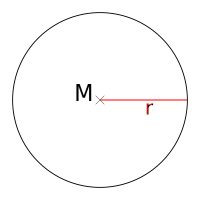
\includegraphics[width=.4\textwidth]{img/euclidean_circle.png}}\qquad
  \subfloat[][Taxicab-Kreis]{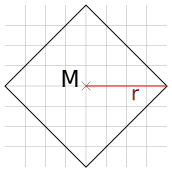
\includegraphics[width=.4\textwidth]{img/taxicab_circle.png}}\\
  \caption{Alle Punkte auf der Kreislinie haben den gleichen Abstand zum Mittelpunkt.
  Auffallend ist, das der Kreis in Taxicab-Metrik nicht rund, sondern quadratisch ist.}
  \label{img:circle_in_diff_metrics}
\end{figure}

Die Berechnung von Mittelpunkt und Radius eines Taxicab-Kreises ist schwieriger als in euklidischer 
Geometrie. Es wird hier keine Formel benutzt, sondern ein Algorithmus. Interessant hier ist das Berechnen
von einem Kreis in Taxicab-Geometrie von zwei oder drei Punkten. Das Problem lässt sich auch wie folgt
beschreiben: Finde das kleinste Quadrat, welches um \unit[45]{\textdegree} gedreht ist, welches zwei (drei) Punkte 
enthält. Da es nicht eindeutig definiert wird, reicht eine einzige Lösung für dieses Problem.

\begin{algorithm}[H]
    \caption{Kreis von zwei Punkten in Taxicab-Geometrie}
    \KwData{Zwei Punkte $X, Y \in \mathbb{R}^n$ }
    \KwResult{Radius und Mittelpunkt eines Quadrates, das $X$ und $Y$ enthält und eine minimale Seitenlänge hat.
    Radius hier ist die halbe Länge der Diagonale.}
    \BlankLine
    \begin{enumerate}
    \item Um die Lösung des Problems zu vereinfachen, werden die Punkte je um \unit[45]{\textdegree} um den
    Ursprung herum gedreht, dann das Quadrat berechnet, die so enstandende Lösung schließlich zurückgedreht.
    \item Rotiere $X, Y$ \unit[45]{\textdegree} um den Ursprung und nenne die so entstehenden Punkte $P, Q$.
    \item Offensichtlich ist nun die Seitenlänge $s$ des minimalen Quadrates gegeben durch
    \begin{equation}
    s = \max\{|P_x - Q_x|, |P_y - Q_y|\}
    \end{equation}
    \item Um eine Lösung zu finden, wähle die unterste linke Ecke als Ausgangspunkt und nenne sie $A$.
    \begin{equation}
    \begin{cases}
    A_x = \min\{P_x,Q_x\}\\
    A_y = \min\{P_y,Q_y\}
    \end{cases}
    \end{equation}
    \item Der rotierte Mittelpunkt $M'$ ist somit gegeben durch
    \begin{equation}
    \begin{cases}
    M'_x = A_x + \frac{s}{2}\\
    M'_y = A_y + \frac{s}{2}
    \end{cases}
    \end{equation}
    \item Rotiere $M'$ um \unit[45]{\textdegree} um den Ursprung und nenne den so entstehenden Punkt $M$.
    \item Der Radius $r$ ist gegeben durch 
    \begin{equation}
    r = \sqrt{A_x - M'_x) ^ 2 + (A_y - M'_y) ^ 2 }
    \end{equation}
    \end{enumerate}
    \Return{$r$, $M$}
\end{algorithm} 

\begin{figure}[!ht]
  \centering
  \subfloat[][Zwei Punkte]{\includegraphics[width=.45\textwidth]{img/taxicab_from_two.png}}\qquad
  \subfloat[][Drei Punkte]{\includegraphics[width=.45\textwidth]{img/taxicab_from_three.png}}\qquad
  \caption{Kreis in Taxicab-Geometrie von zwei respektiv drei Punkten. Auffallend ist, dass mindestens
  zwei Punkte auf der Kreislinie liegen.}
  \label{fig:taxicab_calc}
\end{figure}

Interessanterweise liefert dieser Algorithmus durch geringfügige Anpassungen auch die Lösung für folgendes Problem:
Finde das kleinste Quadrat, welches um \unit[45]{\textdegree} gedreht ist, welches \textbf{drei} Punkte enthält:

\begin{algorithm}[H]
    \caption{Kreis von drei Punkten in Taxicab-Geometrie}
    \KwData{Drei Punkte $X, Y, Z \in \mathbb{R}^n$ }
    \KwResult{Radius und Mittelpunkt eines Quadrates, das $X, Y, Z$ enthält und eine minimale Seitenlänge hat. Radius hier 
    ist die halbe Länge der Diagonale.}
    \BlankLine
    \begin{enumerate}
    \item Um die Lösung des Problems zu vereinfachen, werden die Punkte je um \unit[45]{\textdegree} um den
    Ursprung herum gedreht, dann das Quadrat berechnet, die so enstandende Lösung schließlich zurückgedreht.
    \item Rotiere $X, Y, Z$ \unit[45]{\textdegree} um den Ursprung und nenne die so entstehenden Punkte $P, Q, R$.
    \item Offensichtlich ist nun die Seitenlänge $s$ des minimalen Quadrates gegeben durch
    \begin{equation}
    s = \max\{|P_x-Q_x|,|P_x-R_x|,|Q_x-R_x|,|P_y-Q_y|,|P_y-R_y|,|Q_y-R_y|\}
    \end{equation}
    \item Um eine Lösung zu finden, wähle die unterste linke Ecke als Ausgangspunkt und nenne sie $A$.
    \begin{equation}
    \begin{cases}
    A_x = \min\{P_x,Q_x,R_x\}\\
    A_y = \min\{P_y,Q_y,R_y\}
    \end{cases}
    \end{equation}
    \item Der rotierte Mittelpunkt $M'$ ist somit gegeben durch
    \begin{equation}
    \begin{cases}
    M'_x = A_x + \frac{s}{2}\\
    M'_y = A_y + \frac{s}{2}
    \end{cases}
    \end{equation}
    \item Rotiere $M'$ um \unit[45]{\textdegree} um den Ursprung und nenne den so entstehenden Punkt $M$.
    \item Der Radius $r$ ist gegeben durch 
    \begin{equation}
    r = \sqrt{A_x - M'_x) ^ 2 + (A_y - M'_y) ^ 2 }
    \end{equation}
    \end{enumerate}
    \Return{$r$, $M$}
\end{algorithm}

Im Rahmen dieser Arbeit wurden diese Algorithmen auch mittels GeoGebra visualisiert. Eine interaktive Visualisierung
für einen Kreis in Taxicab-Geometrie, der zwei (drei) Punkte enthält, ist unter folgenden Links zu sehen: 

\url{http://www.geogebratube.org/student/m65241} \newline
\url{http://www.geogebratube.org/student/m68655}

Interessanterweise funktioniert \texttt{minidisk} auch mit Taxicab-Kreisen, wenn man die \texttt{disk}-Funktion anpasst. Dies wurde hier nicht mathematisch bewiesen, aber die Ergebnisse sprechen für sich.

\begin{figure}[!ht]
  \centering
  \includegraphics[width=.9\textwidth]{img/taxicab_minidisk.png}
  \caption{Platzierung von 100 Punkten und deren kleinster umschließender Kreis in Taxicab-Geometrie.}
  \label{img:taxicab_minidisk}
\end{figure}

%#
\section{Zeitbeschränkung}

% ############################################
\clearpage
\section{Implementierung}


% ############################################
\clearpage
\section{Diskussion}

\subsection{Performance}

\subsection{Fehlerrechnung}

\subsubsection{Abweichung vom Optimum}

\subsubsection{Fehler durch Modellierung}

\begin{figure}[!ht]
  \centering
  \subfloat[][]{\includegraphics[width=.4\textwidth, angle=0]{img/collected_edges.png}} \qquad
  \subfloat[][]{\includegraphics[width=.4\textwidth, angle=90]{img/collected_edges.png}}\\
  \subfloat[][]{\includegraphics[width=.4\textwidth, angle=180]{img/collected_edges.png}} \qquad
  \subfloat[][]{\includegraphics[width=.4\textwidth, angle=270]{img/collected_edges.png}}
  \caption{Überstreichen der Ecken beim Wechseln in eine benachbarte Zelle: Der Roboter (hier rot),
  kann nicht nur den ursprünglichen, kreisförmigen Teil in der Mitte einer Zelle abernten, 
  sondern beim Wechseln auch die Ecken, da sein Arbeitsbereich diese in der Bewegung überschneidet. }
  \label{fig:harvested_edges}
\end{figure}

\subsection{Lessons learned/Fehlentscheidungen}

\begin{itemize}
\item Zu viele Abstraktion, die sich später unnötig herausgetsellt hat (Geometry, Circle)
\end{itemize}

\subsection{Ausblick}

\nocite{*}

\printbibliography[maxnames=25]



\end{document}
